\documentclass[11pt,t,usepdftitle=false,aspectratio=169]{beamer}
\usetheme[url]{uibk}

\title[Probability Distribution Forecasts]{Probability Distribution Forecasts: Learning with
  \\\vspace{.2em} Random Forests and Graphical Assessment}
\author[Moritz N. Lang]{Moritz N.\ Lang, Reto Stauffer, Lisa Schlosser, Achim Zeileis}

%-------------------------------------------------------------------
% Preamble
%-------------------------------------------------------------------
%% Create new footer line
% \setbeamertemplate{footline}{
%   \hfill \vspace*{1.em}  \insertframenumber{} / \inserttotalframenumber \hspace*{1ex} {\tiny \ccLogo \ccAttribution} \hspace*{2ex}
% }

\setbeamertemplate{footline}{
 \hspace{1em} \vspace*{1.em} {\tiny \ccLogo \ccAttribution}  \hspace*{1ex} \insertframenumber{} / \inserttotalframenumber \hspace*{2ex}
}

%% Adapt URL font and set URL
\setbeamerfont{url}{size*={11.5pt}{13pt},series=\mdseries}
\URL{https://topmodels.R-Forge.R-project.org/}

%% Adapt headerimage
% \renewcommand{\headerimage}[1]{%
%    \IfStrEqCase{#1}{%
%       {1}{%
%          \gdef\myheaderimageid{#1}%
%          \gdef\myheaderimageposition{nw}%
%          \gdef\myheaderimage{forest.jpg}%
%       }}[%
%          \gdef\myheaderimageid{1}%
%          \gdef\myheaderimageposition{nw}%
%          \gdef\myheaderimage{forest.jpg}%
%       ]%
% }
\headerimage{1}

%% Add graphics path
\graphicspath{{Figures/}}

%% Use some packages
\usepackage[utf8]{inputenc}
\setbeamertemplate{caption}{\insertcaption} 
% \usepackage{Sweave}
\usepackage{changepage}
\usepackage{amsmath,tikz}
\usepackage{calc}
\usepackage{graphicx}
\usetikzlibrary{positioning,shapes,arrows,decorations.pathreplacing,calc,automata,mindmap,trees,tikzmark,decorations.pathreplacing}
\usepackage{xcolor}
\usepackage{fontawesome}
\usepackage{ccicons}

%% Define some new commands
\newcommand{\credit}[1]{\par\hfill \tiny  \ccCopy ~\itshape#1}
\newcommand{\argmax}{\operatorname{argmax}\displaylimits}

%% Create appendix with no page numbering
\newcommand{\backupbegin}{
   \newcounter{finalframe}
   \setcounter{finalframe}{\value{framenumber}}
}
\newcommand{\backupend}{
   \setcounter{framenumber}{\value{finalframe}}
}

%% Define colors
\definecolor{HighlightOrange}{rgb}{0.9490196,0.5725490,0.0000000}
\definecolor{HighlightBlue}{rgb}{0.4784314,0.7490196,0.9803922}
\definecolor{forestred}{RGB}{206,73,81}
\definecolor{treegreen}{RGB}{0,143,0}
\definecolor{lightblue}{RGB}{34,151,230}
\definecolor{lightorange}{RGB}{255,165,0}

%% Sweave options and setup R



%-------------------------------------------------------------------
% Main
%-------------------------------------------------------------------
\begin{document}


\section{Probability Distribution Forecasts: Learning with Random Forests and Graphical Assessment}

%-------------------------------------------------------------------
\subsection{Motivation}
%-------------------------------------------------------------------

%% SLIDE
\begin{frame}%[fragile]
\frametitle{Motivation}
\vspace{-0.41cm}
\begin{figure}[!htb]
\minipage{0.285\textwidth}
\begin{center}
\visible<2->{
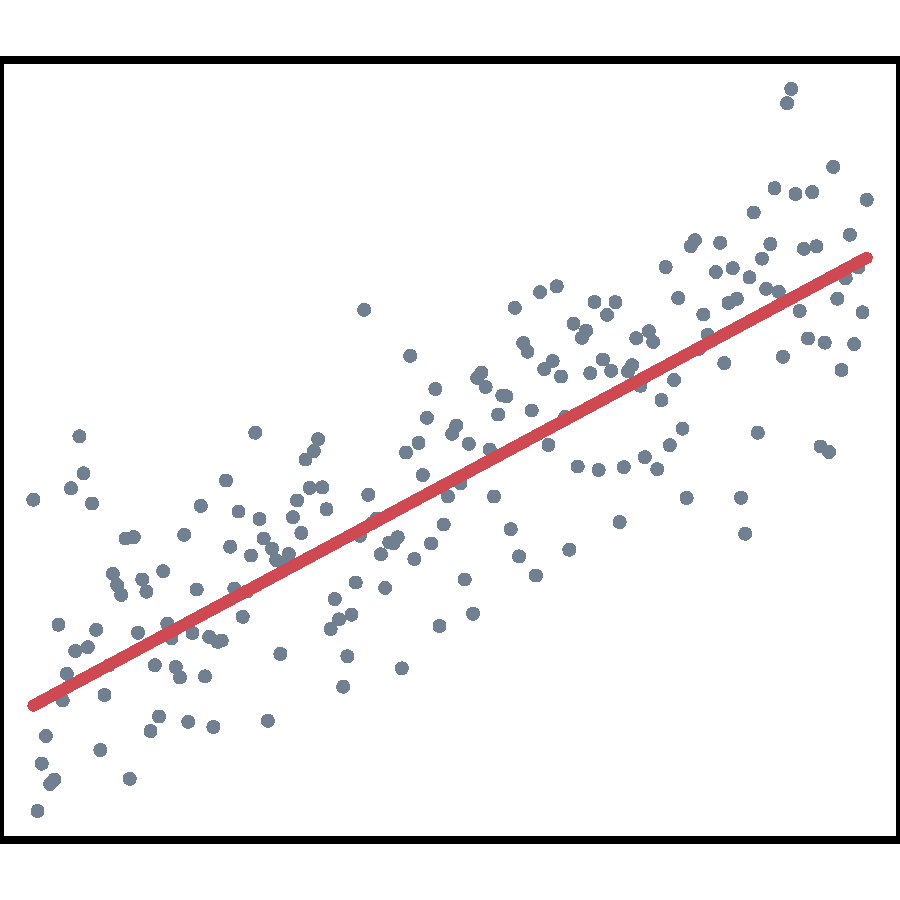
\includegraphics{slides-plot_motivation_GLM}
}
\end{center}
\endminipage
\visible<3->{{\LARGE$\rightarrow$}}
\minipage{0.285\textwidth}
\begin{center}
\visible<3->{
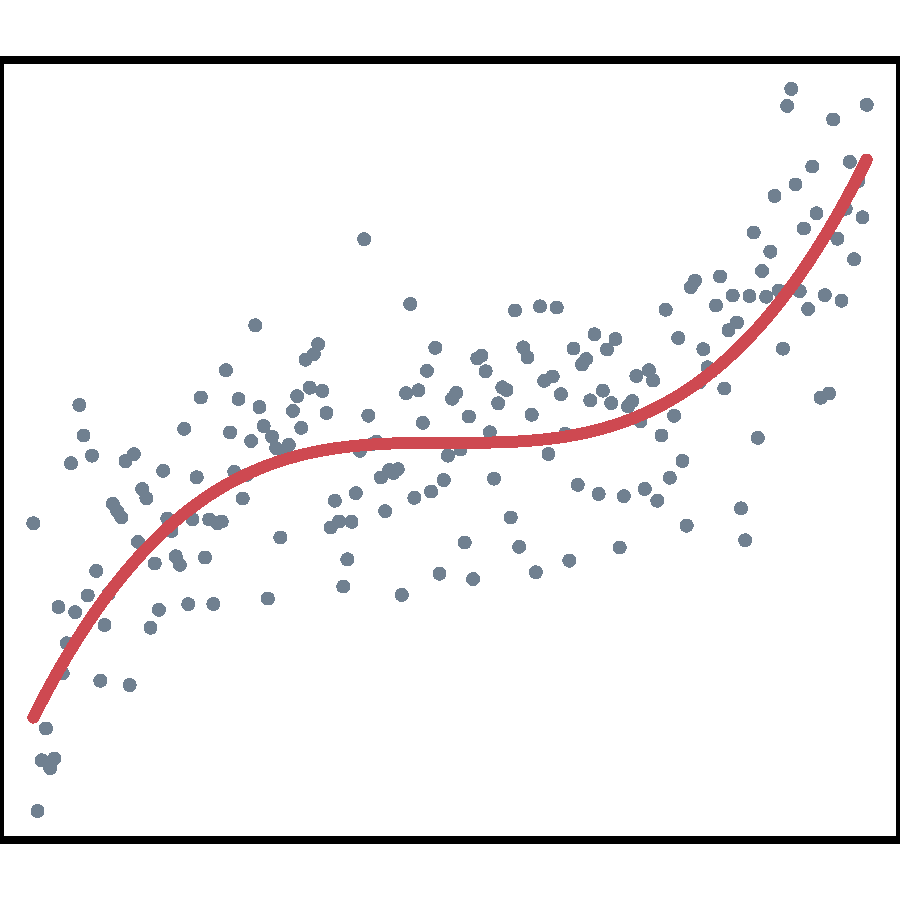
\includegraphics{slides-plot_motivation_GAM}
}
\end{center}
\endminipage
\visible<4->{{\LARGE$\rightarrow$}}
\minipage{0.285\textwidth}
\begin{center}
\visible<4->{
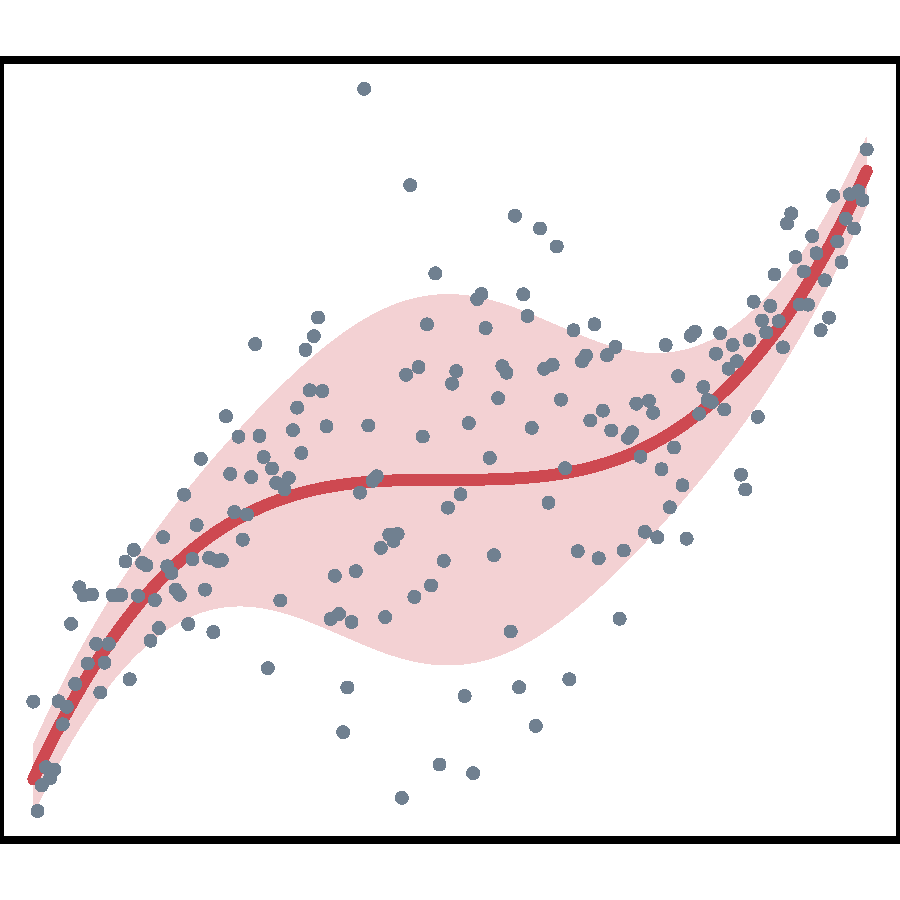
\includegraphics{slides-plot_motivation_GAMLSS}
}
\end{center}
\endminipage

\vspace{0.5cm}
\minipage{0.25\textwidth}
\begin{center}
\visible<2->{
LM, GLM\\
\vspace{0.5cm}
\code{lm}\\
\code{glm}\\
\vspace{1.5cm}}
\end{center}
\endminipage
\hspace{1.1cm}
\minipage{0.25\textwidth}
\begin{center}
\visible<3->{
GAM\\
\vspace{0.5cm}
\code{mgcv}\\
\code{VGAM}\\
\vspace{1.5cm}}
\end{center}
\endminipage
\hspace{1.1cm}
\minipage{0.25\textwidth}
\begin{center}
\visible<4->{
GAMLSS\\
\vspace{0.5cm}
\code{gamlss}\\
\code{mgcv}\\
\code{VGAM}\\
\code{gamboostLSS}\\
\code{bamlss}}
\end{center}
\endminipage
\end{figure}
\end{frame}


%% SLIDE
\begin{frame}[fragile]
\frametitle{Motivation}
\vspace{-0.41cm}
\begin{figure}[!htb]
\minipage{0.285\textwidth}
\begin{center}
\visible<1->{
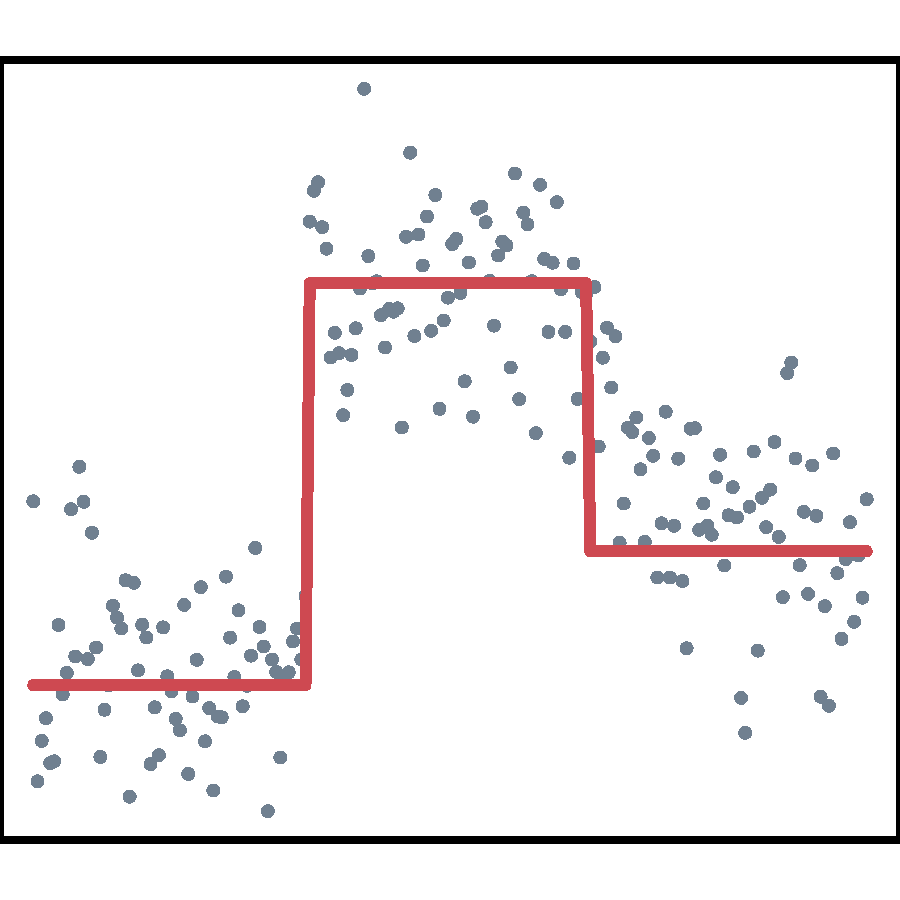
\includegraphics{slides-plot_motivation_regtree}
}
\end{center}

\endminipage
\visible<2->{{\LARGE$\rightarrow$}}
\minipage{0.285\textwidth}
 \begin{center}
\visible<2->{
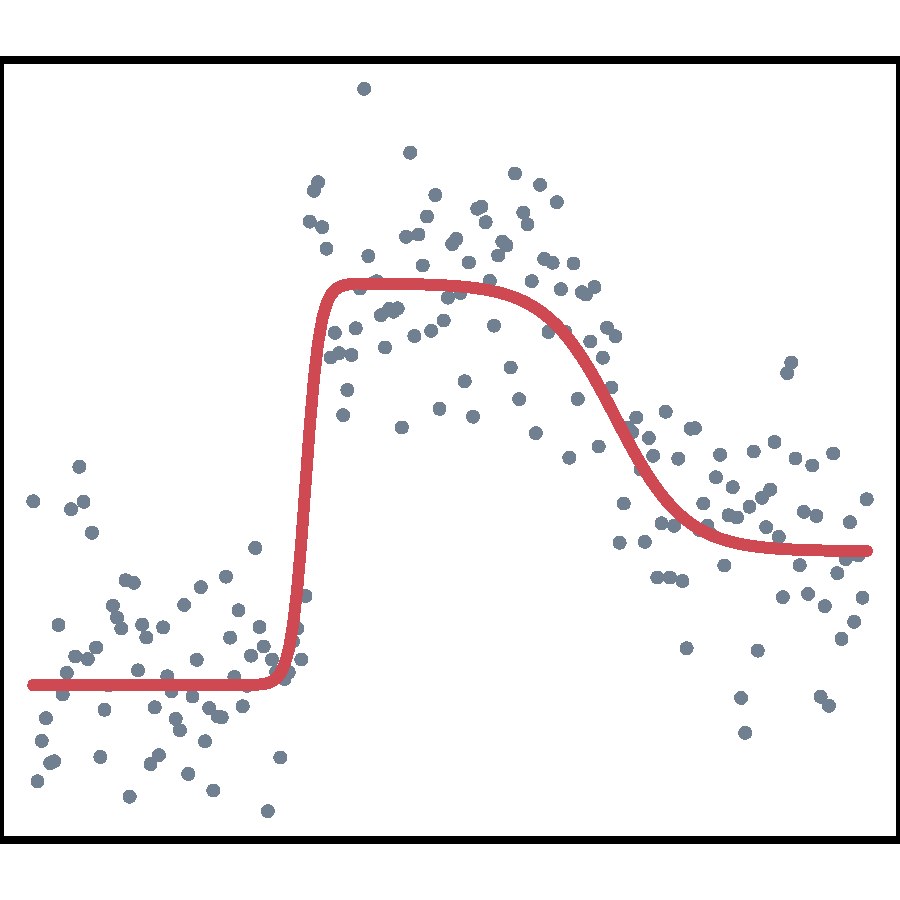
\includegraphics{slides-plot_motivation_randforest}
}
\end{center}

\endminipage
\visible<3->{{\LARGE$\rightarrow$}}
\minipage{0.285\textwidth}
\begin{center}
\visible<3->{

\includegraphics{slides-plot_motivation_question}
}
\end{center}

\endminipage

\minipage{0.285\textwidth}
\begin{center}
\vspace{0.0cm}
\visible<1->{
Regression tree\\
\vspace{0.3cm}
\resizebox{0.2\textwidth}{!}{
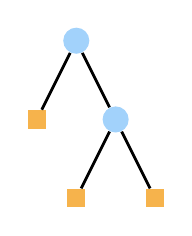
\begin{tikzpicture}
  \node[ellipse, fill=HighlightBlue!70, align=center] (n0) at (1, 2) {};
  \node[rectangle, fill=HighlightOrange!70, align=center] (n1) at (0.5, 1) {};
  \draw[-, line width=1pt] (n0) -- (n1);
  \node[ellipse, fill=HighlightBlue!70, align=center] (n2) at (1.5, 1) {};
  \draw[-, line width=1pt] (n0) -- (n2);
  \node[rectangle, fill=HighlightOrange!70, align=center] (n3) at (1, 0) {};
  \draw[-, line width=1pt] (n2) -- (n3);
  \node[rectangle, fill=HighlightOrange!70, align=center] (n4) at (2, 0) {};
  \draw[-, line width=1pt] (n2) -- (n4);
\end{tikzpicture}}
\vspace{0.2cm}\\
\code{rpart}\\
\code{party(kit)}\\
\vspace{1cm}}
\end{center}
\endminipage
\hspace{0.65cm}
\minipage{0.285\textwidth}
\begin{center}
\vspace{-0.4cm}
\visible<2->{
Random forest\\
\vspace{0.4cm}
\resizebox{0.6\textwidth}{!}{
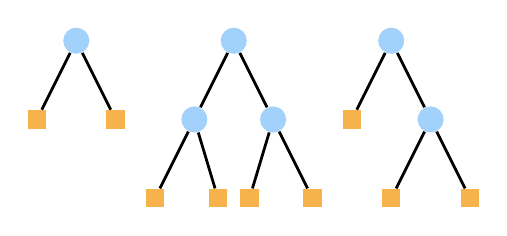
\begin{tikzpicture}
  \node[ellipse, fill=HighlightBlue!70, align=center] (n00) at (1, 2) {};
  \node[rectangle, fill=HighlightOrange!70, align=center] (n01) at (0.5, 1) {};
  \draw[-, line width=1pt] (n00) -- (n01);
  \node[rectangle, fill=HighlightOrange!70, align=center] (n02) at (1.5, 1) {};
  \draw[-, line width=1pt] (n00) -- (n02);
  
  \node[ellipse, fill=HighlightBlue!70, align=center] (n10) at (3, 2) {};
  \node[ellipse, fill=HighlightBlue!70, align=center] (n11) at (2.5, 1) {};
  \draw[-, line width=1pt] (n10) -- (n11);
  \node[ellipse, fill=HighlightBlue!70, align=center] (n12) at (3.5, 1) {};
  \draw[-, line width=1pt] (n10) -- (n12);
  \node[rectangle, fill=HighlightOrange!70, align=center] (n13) at (2, 0) {};
  \draw[-, line width=1pt] (n11) -- (n13);
  \node[rectangle, fill=HighlightOrange!70, align=center] (n14) at (2.8, 0) {};
  \draw[-, line width=1pt] (n11) -- (n14);
  \node[rectangle, fill=HighlightOrange!70, align=center] (n15) at (3.2, 0) {};
  \draw[-, line width=1pt] (n12) -- (n15);
  \node[rectangle, fill=HighlightOrange!70, align=center] (n16) at (4, 0) {};
  \draw[-, line width=1pt] (n12) -- (n16);
  
  \node[ellipse, fill=HighlightBlue!70, align=center] (n20) at (5, 2) {};
  \node[rectangle, fill=HighlightOrange!70, align=center] (n21) at (4.5, 1) {};
  \draw[-, line width=1pt] (n20) -- (n21);
  \node[ellipse, fill=HighlightBlue!70, align=center] (n22) at (5.5, 1) {};
  \draw[-, line width=1pt] (n20) -- (n22);
  \node[rectangle, fill=HighlightOrange!70, align=center] (n23) at (5, 0) {};
  \draw[-, line width=1pt] (n22) -- (n23);
  \node[rectangle, fill=HighlightOrange!70, align=center] (n24) at (6, 0) {};
  \draw[-, line width=1pt] (n22) -- (n24);
\end{tikzpicture}
}
\vspace{0.3cm}\\
\code{randomForest}\\
\code{ranger}\\
\code{party(kit)}}
\end{center}
\endminipage
\hspace{0.65cm}
\minipage{0.285\textwidth}
\begin{center}
\vspace{0.15cm}
\visible<3->{
Distributional trees and forests\\
\vspace{1.15cm}
\code{disttree}\\
based on \code{partykit}\\
\vspace{1cm}}
\end{center}
\endminipage
\end{figure}
\end{frame}


%% SLIDE
\begin{frame}
\frametitle{Motivation}

\vspace{-0.75em}

\textbf{Distributional:}
\begin{itemize}
  \item Specify the complete probability distribution (location, scale, shape, \dots).
\end{itemize}

\medskip

\textbf{Tree:}
\begin{itemize}
  \item Automatic detection of steps and abrupt changes. %(data driven)
  \item Capture non-linear and non-additive effects and interactions.
\end{itemize}

\medskip

\textbf{Forest:}
\begin{itemize}
  \item Smoother effects.
  \item Stabilization and regularization of the model.
\end{itemize}
\end{frame}

%-------------------------------------------------------------------
\subsection{Learning}
%-------------------------------------------------------------------
%% SLIDE
\begin{frame}
   \frametitle{Learning distributional trees and forests}
      \begin{minipage}{0.7\textwidth}
   \vspace{-0.45em}
      {\bf Tree:}
      \begin{enumerate}
      \item<3-> Fit global distributional model $\mathcal{D}(Y; \theta)$: \\ % to the whole data set:\\
      Estimate model parameters $\hat{\theta}$.
      \item<7-> Evaluate goodness of fit \\
      (for each parameter and each observation).
      \item<8-> Choose covariate $X$ with strongest influence on goodness of fit
        of $\mathcal{D}(Y; \hat{\theta})$ as split variable.
      \item<8-> Find the split point $p$ which leads to the highest improvement.
      \item<10-> Repeat steps 1--4 recursively in the subgroups
        until some stopping criterion is met.
      \end{enumerate}
    \vspace{0.05cm}
      \visible<13->{
      {\bf Forest:} Ensemble of $T$ trees.
      \begin{itemize}
      \item Bootstrap or subsamples.
      \item Random input variable sampling.
      \end{itemize}
      }
      \end{minipage}
      \begin{minipage}{0.23\textwidth}
      \vspace{-3.45cm}
      \begin{tikzpicture}
      \visible<2-3>{
      \node[ellipse, fill=HighlightBlue!70, align=center, scale = 0.7, minimum width=71pt, minimum height = 30pt] (n0) at (0.8, 1.7) {$Y$};
      }
      \visible<4>{
      \node[ellipse, fill=HighlightBlue!70, align=center, scale = 0.7, minimum width=71pt, minimum height = 30pt] (n0) at (0.8, 1.7) {$\mathcal{D}(Y;\hat{\theta}$)};
      }
      \visible<5->{
      \node[inner sep=0pt] (density_root) at (0.8, 1.7)
          {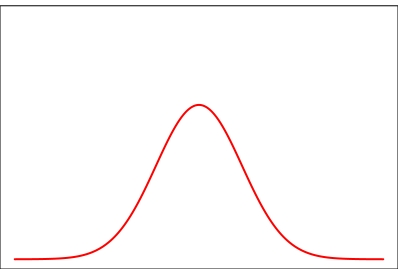
\includegraphics[width=0.6\textwidth]{density1.jpeg}};
      }
      \visible<6-8>{
      \node[rectangle, fill=HighlightOrange!70, align=center, scale = 0.7, minimum width=60pt, minimum height = 20pt] (n1) at (0, 0) {?};
      \node[rectangle, fill=HighlightOrange!70, align=center, scale = 0.7, minimum width=60pt, minimum height = 20pt] (n2) at (1.6, 0) {?};
      \draw[-, gray, line width=0.5pt] (0.7, 1) -- (n1);
      \draw[-, gray, line width=0.5pt] (0.9, 1) -- (n2);
      }
      \visible<9-10>{
      \node[rectangle, fill=HighlightOrange!70, align=center, scale = 0.7, minimum width=60pt, minimum height = 20pt] (n1) at (0, 0) {$Y_1$};
      \node[rectangle, fill=HighlightOrange!70, align=center, scale = 0.7, minimum width=60pt, minimum height = 20pt] (n2) at (1.6, 0) {$Y_2$};
      \draw[-, gray, line width=0.5pt] (0.7, 1) -- (n1) node [midway, left] {\scriptsize $X \leq p$};
      \draw[-, gray, line width=0.5pt] (0.9, 1) -- (n2) node [midway, right] {\scriptsize $X > p$};
      }
      \visible<11>{
      \node[rectangle, fill=HighlightOrange!70, align=center, scale = 0.7, minimum width=60pt, minimum height = 20pt] (n1) at (0, 0) {$\mathcal{D}(Y_1;\hat{\theta}_1$)};
      \node[rectangle, fill=HighlightOrange!70, align=center, scale = 0.7, minimum width=60pt, minimum height = 20pt] (n2) at (1.6, 0) {$\mathcal{D}(Y_2;\hat{\theta}_2$)};
      }
      \visible<11->{
      \draw[-, gray, line width=0.5pt] (0.7, 1) -- (n1) node [midway, left] {\scriptsize $X \leq p$};
      \draw[-, gray, line width=0.5pt] (0.9, 1) -- (n2) node [midway, right] {\scriptsize $X > p$};
      }
      \visible<12->{
      \node[inner sep=0pt] (density2) at (-0.1,-0.3)
          {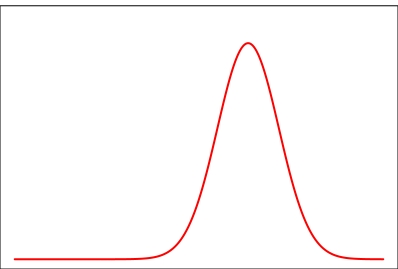
\includegraphics[width=0.5\textwidth]{density2.jpeg}};
      }
      \visible<12->{
      \node[inner sep=0pt] (density3) at (1.7,-0.3)
          {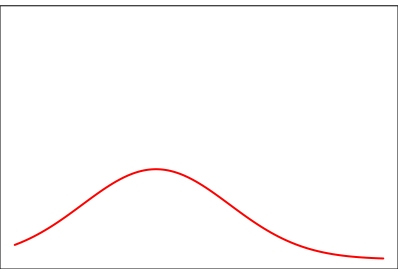
\includegraphics[width=0.5\textwidth]{density3.jpeg}};
      }
      \end{tikzpicture}
      \end{minipage}
      \vspace{0.4cm}
\end{frame}


% %% SLIDE
% \begin{frame}
% \frametitle{Learning distributional trees and forests}
%       \begin{minipage}{1\textwidth}
%    \vspace{-0.45em}
%       {\bf Forests:}
%       \begin{enumerate}
%       \item Learn an ensemble of $T$ trees:\\
%        Each tree is built on a bootstrap or subsample of the data, with
%       random input variable sampling.
%       \item<2-> Aggregate / average over estimated $T$ trees:\\
%       To stabilize and regularize the model.
%       %\item<3-> Only observations $\bold{x}_i$ in the same subgroup as a 
%       %(new) observation $\bold{x}$ enter the parameter estimation.
%       \item<2-> Weighted parameter estimation:\\The weight of observation $i$ for the parameter 
%         estimation for a 
%         (new) observation $j$ is the mean of assignments to the same node.
%       \end{enumerate}
%       \end{minipage}
% \begin{center}
% \minipage{0.38\textwidth}
% \vspace{0.5em}
% \resizebox{0.94\textwidth}{!}{
% \begin{tikzpicture}
%   \visible<3->{
%   \draw (11.1,5) node{\phantom{.}};
%   \draw (18.5,9) node{\phantom{.}};
% 
%   \node[ellipse, fill=HighlightBlue!70, align=center] (n0) at (12, 9) {};
%   \node[rectangle, fill=HighlightOrange!70, align=center] (n1) at (11.5, 8) {\only<4->{$i, j$}};
%   \draw[-, line width=1pt] (n0) -- (n1);
%   \node[ellipse, fill=HighlightBlue!70, align=center] (n2) at (12.5, 8) {};
%   \draw[-, line width=1pt] (n0) -- (n2);
%   \node[rectangle, fill=HighlightOrange!70, align=center] (n3) at (12, 7) {};
%   \draw[-, line width=1pt] (n2) -- (n3);
%   \node[rectangle, fill=HighlightOrange!70, align=center] (n4) at (13, 7) {};
%   \draw[-, line width=1pt] (n2) -- (n4);
%   }
% 
%   \visible<5->{
% 
%   \node[ellipse, fill=HighlightBlue!70, align=center] (n1_0) at (12+3.25, 9) {};
%   \node[ellipse, fill=HighlightBlue!70, align=center] (n1_1) at (11.5+3.25, 8) {};
%   \draw[-, line width=1pt] (n1_0) -- (n1_1);
%   \node[rectangle, fill=HighlightOrange!70, align=center] (n1_2) at (12.5+3.25, 8) {\only<6->{$i, j$}};
%   \draw[-, line width=1pt] (n1_0) -- (n1_2);
%   \node[ellipse, fill=HighlightBlue!70, align=center] (n1_3) at (11+3.25, 7) {};
%   \draw[-, line width=1pt] (n1_1) -- (n1_3);
%   \node[rectangle, fill=HighlightOrange!70, align=center] (n1_4) at (12+3.25, 7) {};
%   \draw[-, line width=1pt] (n1_1) -- (n1_4);
%   \node[rectangle, fill=HighlightOrange!70, align=center] (n1_5) at (10.5+3.25, 6) {};
%   \draw[-, line width=1pt] (n1_3) -- (n1_5);
%   \node[ellipse, fill=HighlightBlue!70, align=center] (n1_6) at (11.5+3.25, 6) {};
%   \draw[-, line width=1pt] (n1_3) -- (n1_6);
%   \node[rectangle, fill=HighlightOrange!70, align=center] (n1_7) at (11+3.25, 5) {};
%   \draw[-, line width=1pt] (n1_6) -- (n1_7);
%   \node[rectangle, fill=HighlightOrange!70, align=center] (n1_8) at (12+3.25, 5) {};
%   \draw[-, line width=1pt] (n1_6) -- (n1_8);
% 
%   \node[ellipse, fill=HighlightBlue!70, align=center] (n2_0) at (12+6, 9) {};
%   \node[ellipse, fill=HighlightBlue!70, align=center] (n2_1) at (11.5+6, 8) {};
%   \draw[-, line width=1pt] (n2_0) -- (n2_1);
%   \node[rectangle, fill=HighlightOrange!70, align=center] (n2_2) at (12.5+6, 8) {};
%   \draw[-, line width=1pt] (n2_0) -- (n2_2);
%   \node[rectangle, fill=HighlightOrange!70, align=center] (n2_3) at (11+6, 7) {\only<6->{$i\vphantom{j}$}};
%   \draw[-, line width=1pt] (n2_1) -- (n2_3);
%   \node[rectangle, fill=HighlightOrange!70, align=center] (n2_4) at (12+6, 7) {\only<6->{$j$}};
%   \draw[-, line width=1pt] (n2_1) -- (n2_4);
%   }
% \end{tikzpicture}
% }
% \endminipage
% \end{center}
% \end{frame}


%-------------------------------------------------------------------
\subsection{Application}
%-------------------------------------------------------------------

%% SLIDE
\begin{frame}[fragile]
\frametitle{Application}

\vspace{-0.75em}

\textbf{Goal:} Probabilistic precipitation forecasting.

\bigskip
\pause

\textbf{Observation data:}
\begin{itemize}
\item Daily 24h precipitation sums from July over 28 years (1985--2012).
\item Observation station ``Axams'' in Tyrol, Austria.
\end{itemize}

\bigskip
\pause

\textbf{Covariates:} 
\begin{itemize}
\item Numeric ensemble weather predictions of precipitation, temperature, air pressure, 
  convective available potential energy, \dots
\item 80 covariates based on ensemble min/max/mean/standard deviation.
\end{itemize}

\bigskip
\pause

\textbf{Distribution assumption:} Power-transformed Gaussian, censored at 0.
\[ (\text{precipitation})^\frac{1}{1.6} \sim \textit{c}\mathcal{N}(\mu,\sigma^2) \]

\end{frame}


%-------------------------------------------------------------------
\subsection{Application}
%-------------------------------------------------------------------

%% R CHUNK FOR NEXT SLIDE

%% SLIDE
\begin{frame}[fragile]
\frametitle{Application}

\vspace{-0.75em}

\textbf{Predictive performance:} Distributional forests improve CRPS skill score compared to heteroscedastic linear model (EMOS) and competing GAMLSS. 

\begin{center}
\vspace{-0.8cm}
\setkeys{Gin}{width=0.65\textwidth}
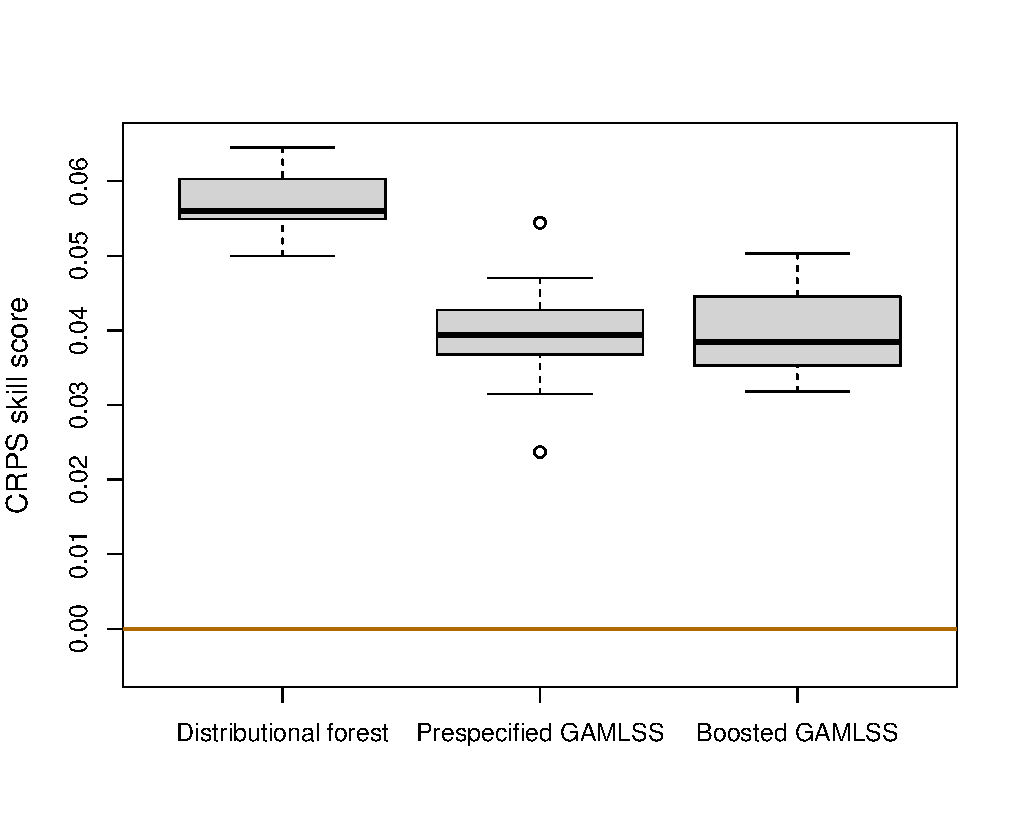
\includegraphics{slides-rain_cross_axams_crps_skills_score}
\end{center}

\end{frame}


%-------------------------------------------------------------------
\subsection{Graphical assessment}
%-------------------------------------------------------------------

%% R CHUNK FOR NEXT SLIDE


%% SLIDE
\begin{frame}[fragile]
\frametitle{Graphical assessment}

\vspace{-0.75em}

\textbf{However:} Is the distributional fit calibrated? 

\bigskip
\pause

\textbf{Graphical assessments:} Various possibilities suggested in different parts of the literature.

\begin{itemize}
  \item (Randomized) quantile-quantile residuals plot.
  \item Probability integral transform (PIT) histogram.
  \item Rootogram.
  \item Reliability diagram at prespecified thresholds.
  \item Worm plot.
\end{itemize}

\bigskip
\pause

\textbf{In R:} Different bits in various packages but no unifying and flexible infrastructure.

\bigskip
\pause

\textbf{Now:} \code{topmodels} (on R-Forge). 


\end{frame}


%% SLIDE
\begin{frame}[fragile]
\frametitle{Graphical assessment}

\vspace{-0.75em}

\textbf{Packages and data:} 

\begin{Schunk}
\begin{Sinput}
R> install.packages("disttree", repos = "https://R-Forge.R-project.org")
R> install.packages("topmodels", repos = "https://R-Forge.R-project.org")
\end{Sinput}
\end{Schunk}
\begin{Schunk}
\begin{Sinput}
R> library("disttree")
R> library("topmodels")
\end{Sinput}
\end{Schunk}
\begin{Schunk}
\begin{Sinput}
R> data("RainAxams", package = "disttree")
\end{Sinput}
\end{Schunk}

\vspace*{1em}

\textbf{Random forest:} 

\begin{Schunk}
\begin{Sinput}
R> forest <- distforest(robs ~ ., 
+                       family = dist_list_cens_normal, 
+                       data = RainAxams, ...)
\end{Sinput}
\end{Schunk}
\end{frame}


%% SLIDE
\begin{frame}[fragile]
\frametitle{Graphical assessment}

\vspace{-0.75em}

\textbf{Q-Q residuals plot:} \code{qqrplot(forest)} 

\vspace{0.25em}

\begin{center}
\setkeys{Gin}{width=0.65\textwidth}
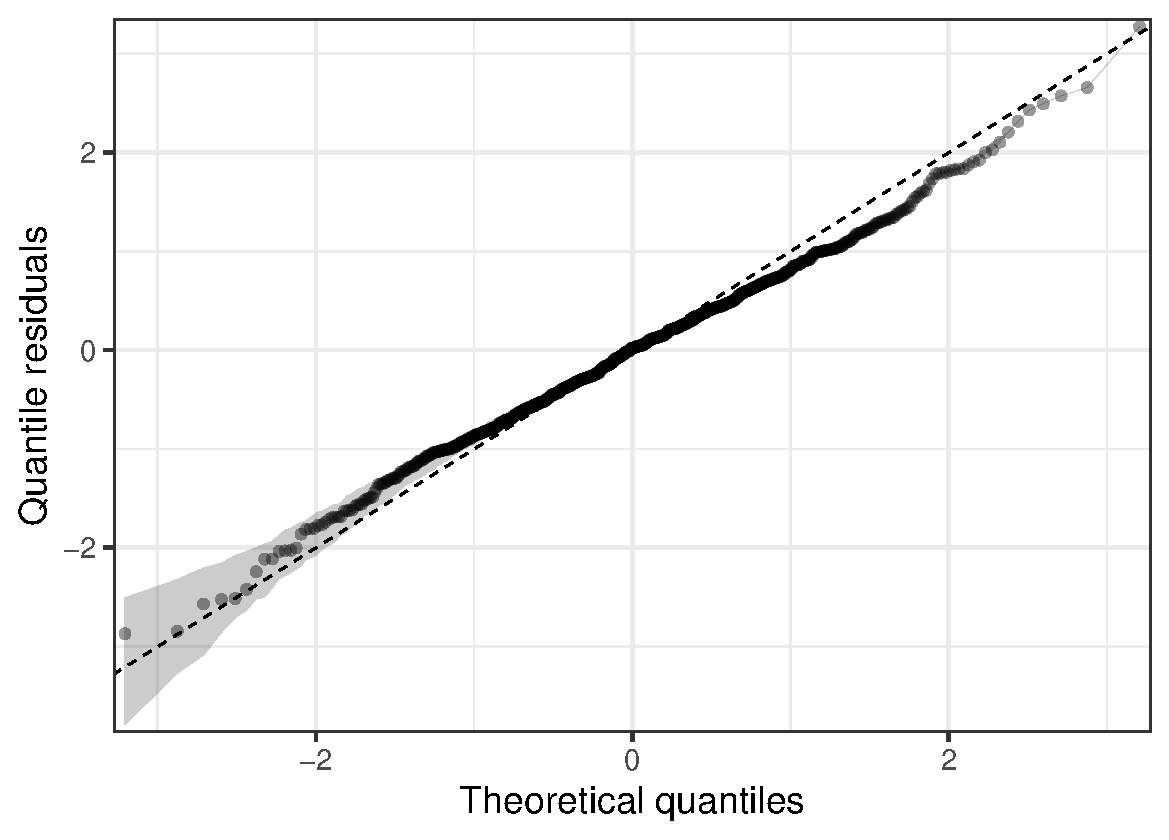
\includegraphics{slides-rain_topmodels_df_qqrplot}
\end{center}
\end{frame}


%% SLIDE
\begin{frame}[fragile]
\frametitle{Graphical assessment}

\vspace{-0.75em}

\textbf{PIT histogram:} \code{pithist(forest)} 

\vspace{0.25em}

\begin{center}
\setkeys{Gin}{width=0.65\textwidth}
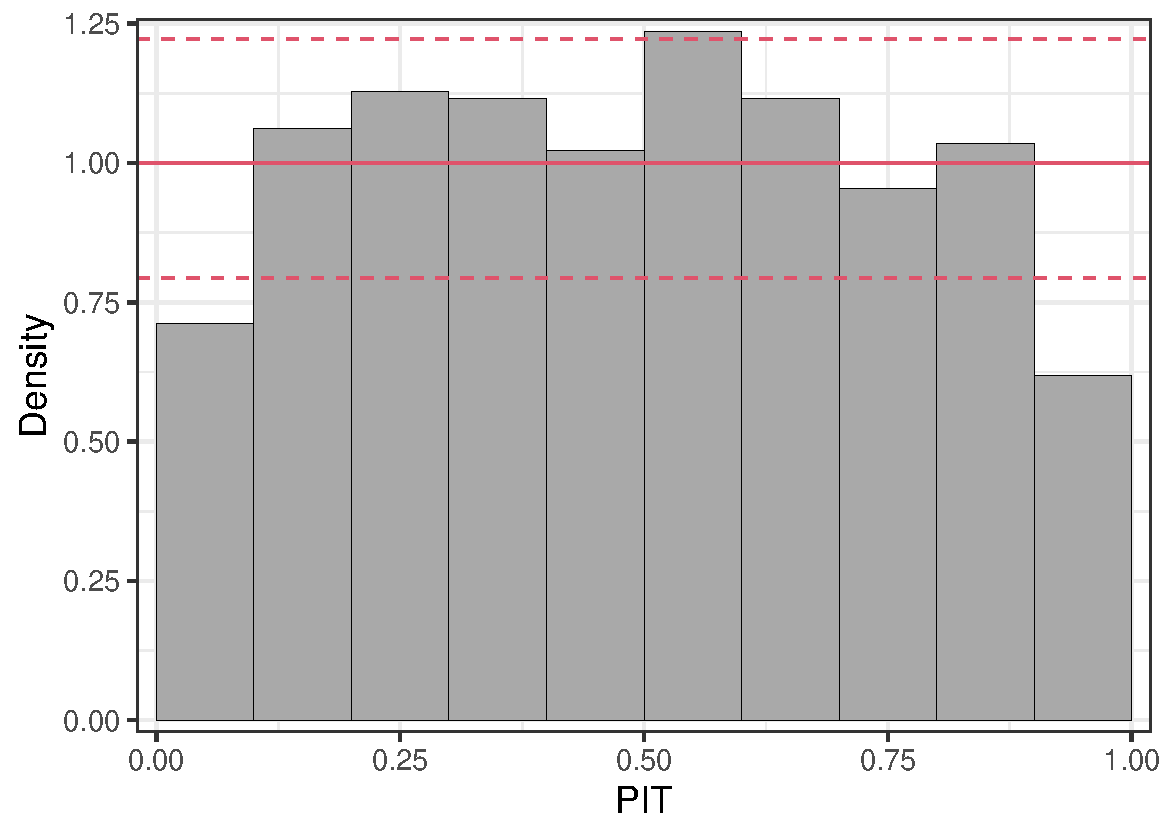
\includegraphics{slides-rain_topmodels_df_pithist}
\end{center}
\end{frame}


%% SLIDE
\begin{frame}[fragile]
\frametitle{Graphical assessment}

\vspace{-0.75em}

\textbf{Rootogram:} \code{rootogram(forest)} 

\vspace{0.25em}

\begin{center}
\setkeys{Gin}{width=0.65\textwidth}
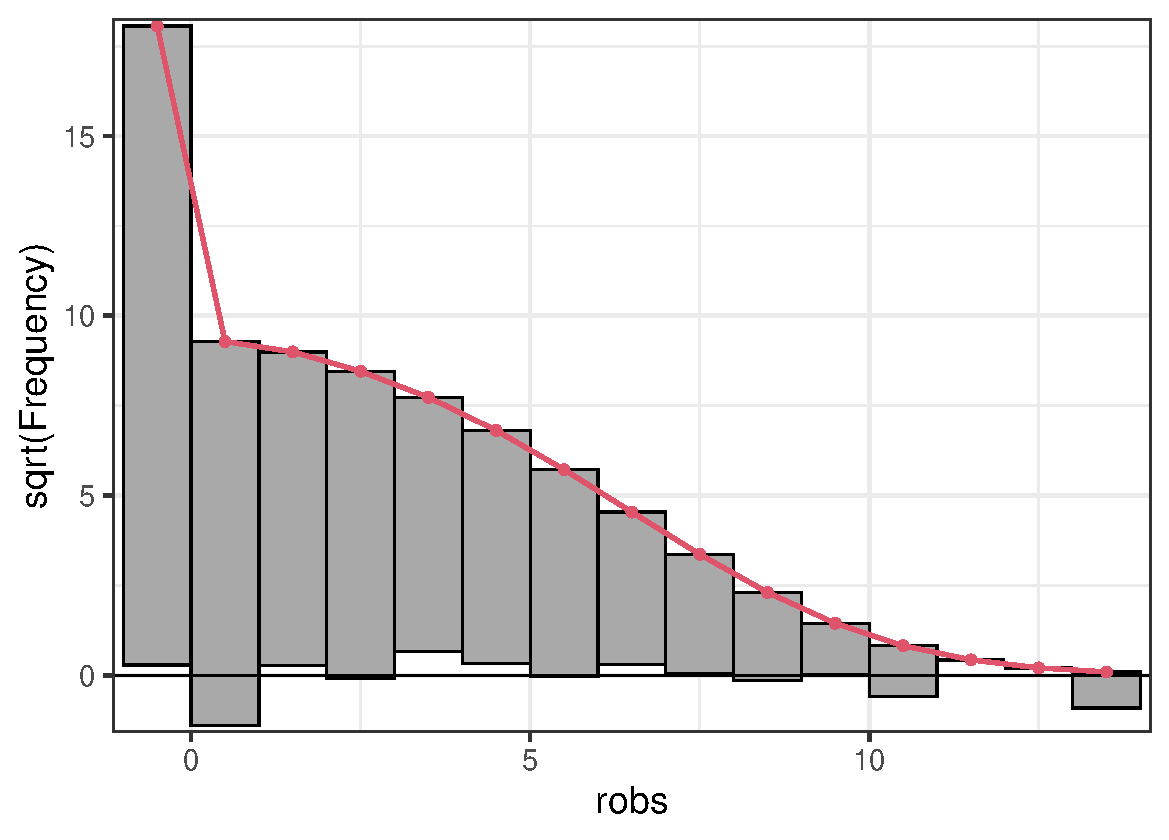
\includegraphics{slides-rain_topmodels_df_rootogram}
\end{center}
\end{frame}


%% SLIDE
\begin{frame}[fragile]
\frametitle{Graphical assessment}

\vspace{-0.75em}

\textbf{Reliability diagram:} \code{reliagram(forest)} 

\vspace{0.25em}

\begin{center}
\setkeys{Gin}{width=0.65\textwidth}
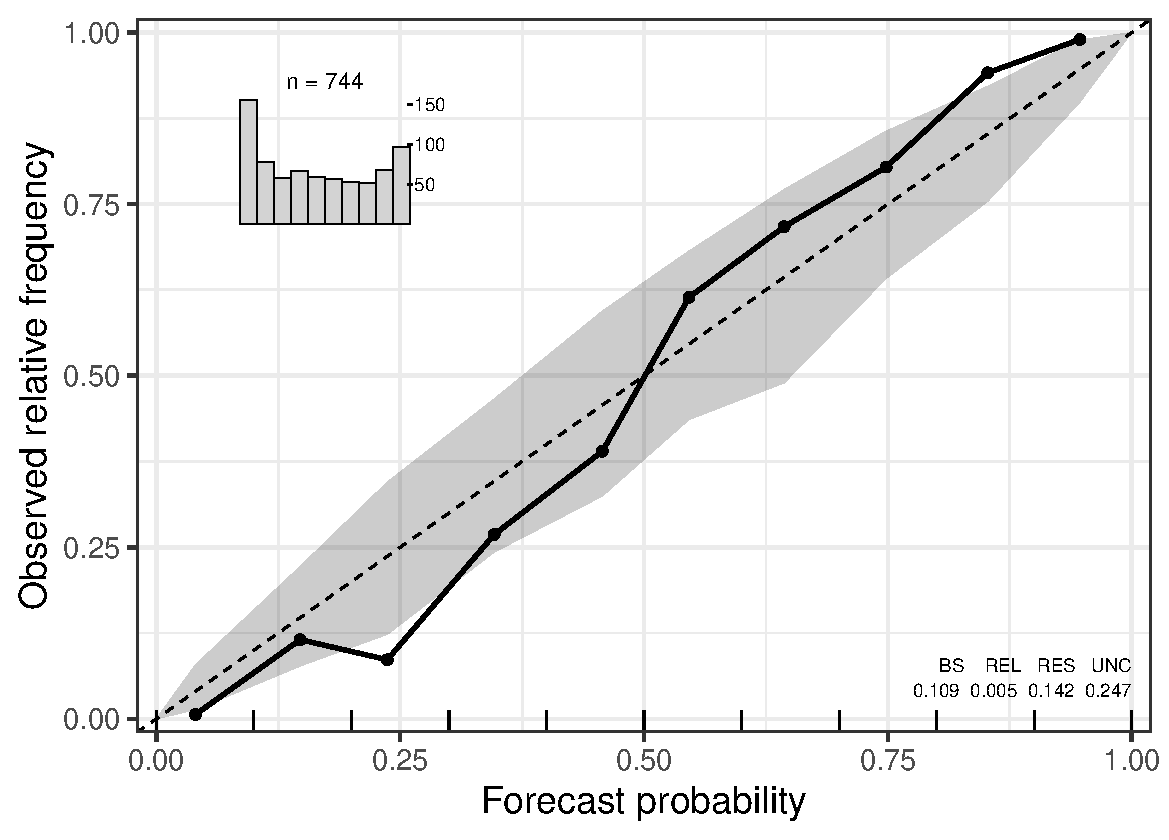
\includegraphics{slides-rain_topmodels_df_reliagram}
\end{center}
\end{frame}


%% SLIDE
\begin{frame}[fragile]
\frametitle{Graphical assessment}

\vspace{-0.75em}

\textbf{Worm plot:} \code{wormplot(forest)} 

\vspace{0.25em}

\begin{center}
\setkeys{Gin}{width=0.65\textwidth}
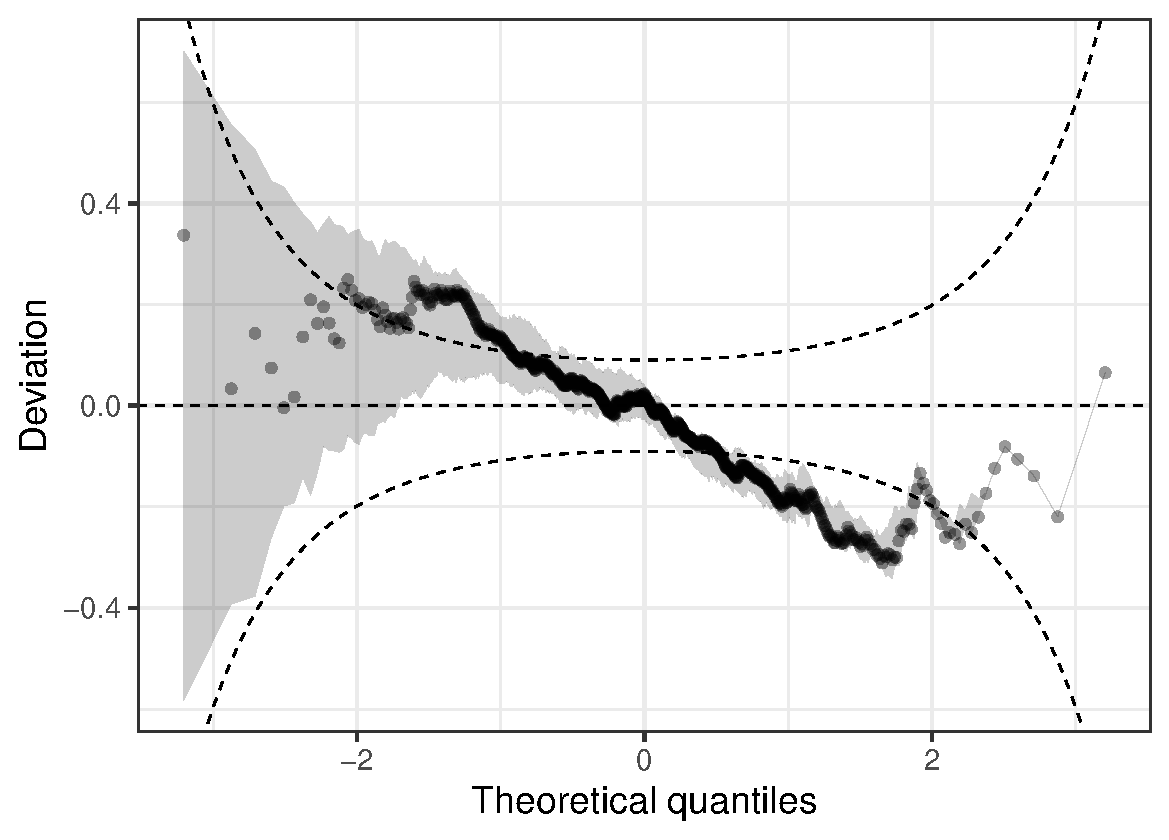
\includegraphics{slides-rain_topmodels_df_wormplot}
\end{center}
\end{frame}


%% SLIDE
\begin{frame}[fragile]
\frametitle{Graphical assessment}

\vspace{-0.75em}

\textbf{In contrast:} Linear Gaussian model.

\begin{itemize}
  \item Homoscedastic.
  \item Not accounting for excess zeros.
  \item Incorrect assumption of underlying response distribution. 
\end{itemize}

\vspace{1em}

\begin{Schunk}
\begin{Sinput}
R> linear <- lm(robs ~ tppow_mean, data = RainAxams)
\end{Sinput}
\end{Schunk}

\end{frame}


%% SLIDE
\begin{frame}[fragile]
\frametitle{Graphical assessment}

\vspace{-0.75em}

\textbf{Model comparison: Rootogram}

\vspace{0.5em}

\begin{Schunk}
\begin{Sinput}
R> rootogram(linear, plot = FALSE) |>
+    autoplot(legend = TRUE)
\end{Sinput}
\end{Schunk}

\begin{center}
\setkeys{Gin}{width=0.65\textwidth}
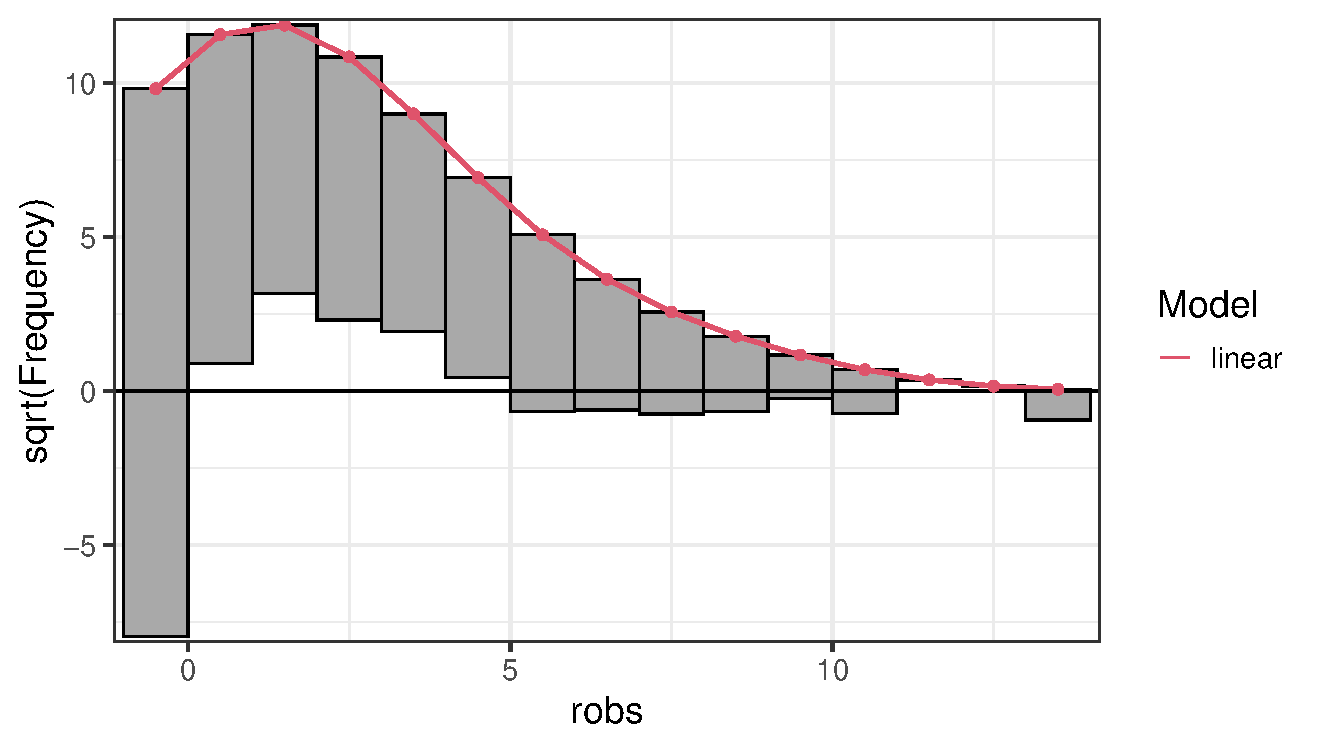
\includegraphics{slides-rain_topmodels_lm_rootogram1}
\end{center}

\end{frame}


%% SLIDE
\begin{frame}[fragile]
\addtocounter{framenumber}{-1}
\frametitle{Graphical assessment}

\vspace{-0.75em}

\textbf{Model comparison: Rootogram}

\vspace{0.5em}

\begin{Schunk}
\begin{Sinput}
R> rootogram(linear, plot = FALSE, breaks = -9:14) |>
+    autoplot(legend = TRUE)
\end{Sinput}
\end{Schunk}

\begin{center}
\setkeys{Gin}{width=0.65\textwidth}
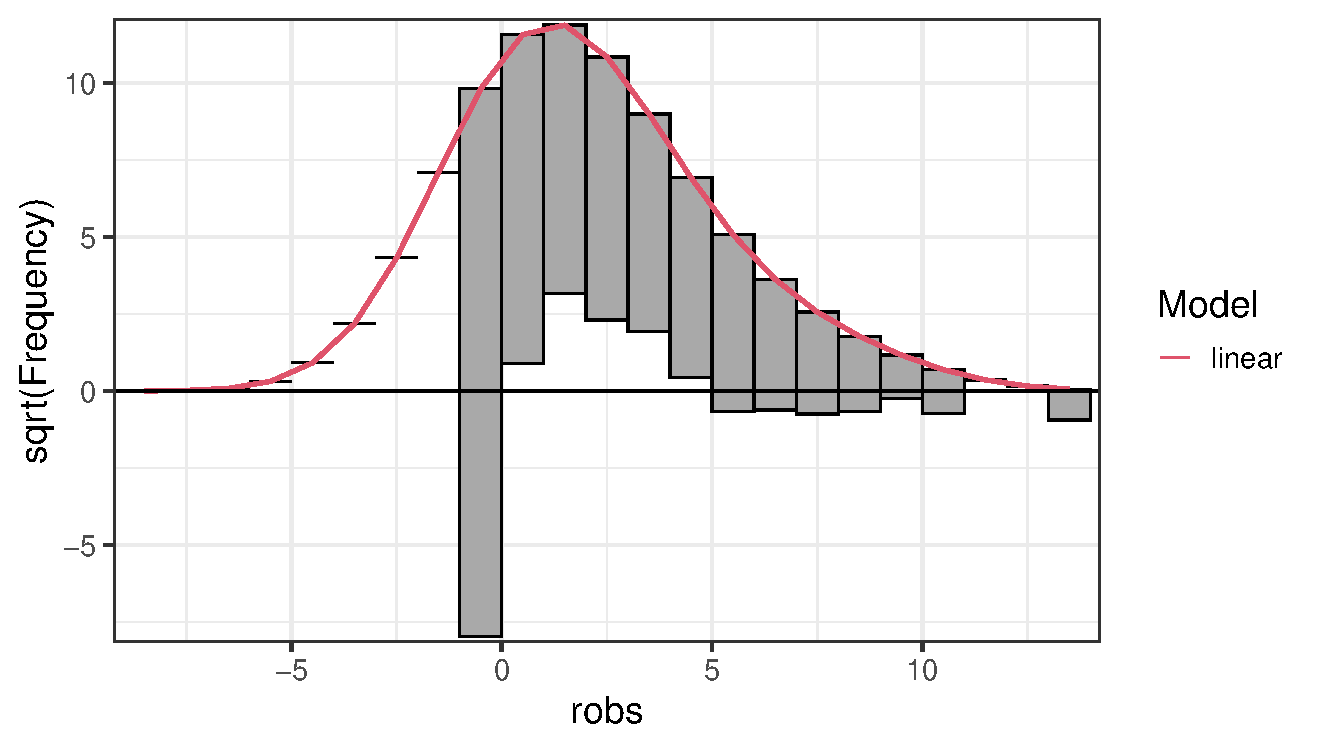
\includegraphics{slides-rain_topmodels_lm_rootogram}
\end{center}

\end{frame}


%% SLIDE
\begin{frame}[fragile]
\addtocounter{framenumber}{-1}
\frametitle{Graphical assessment}

\vspace{-0.75em}

\textbf{Model comparison: Rootogram}

\vspace{0.5em}

\begin{Schunk}
\begin{Sinput}
R> c(rootogram(forest, breaks = -9:14), rootogram(linear, breaks = -9:14)) |>
+    autoplot(legend = TRUE)
\end{Sinput}
\end{Schunk}

\begin{center}
\setkeys{Gin}{width=0.65\textwidth}
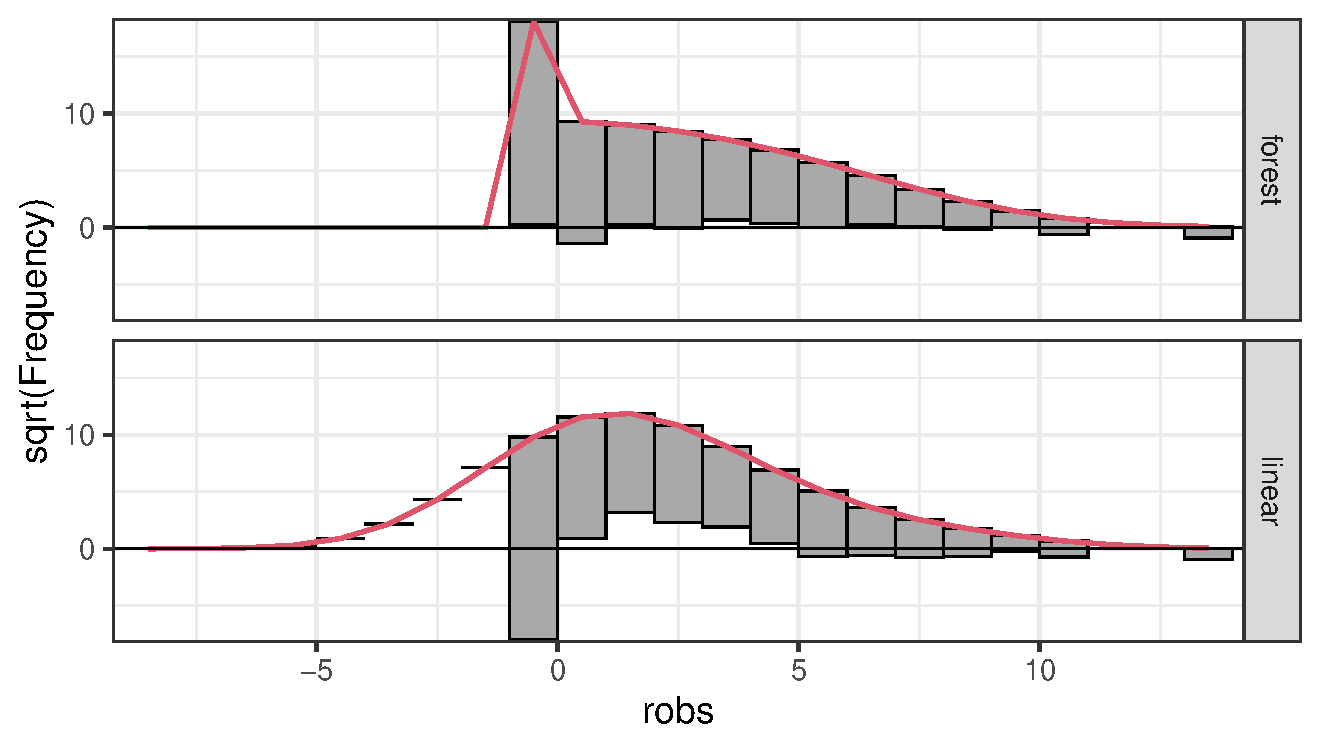
\includegraphics{slides-rain_topmodels_comp_rootogram}
\end{center}

\end{frame}


%% SLIDE
\begin{frame}[fragile]
\frametitle{Graphical assessment}

\vspace{-0.75em}

\textbf{Model comparison: PIT histogram}

\vspace{0.5em}

\begin{Schunk}
\begin{Sinput}
R> pithist(forest, plot = FALSE) |>
+    autoplot(legend = TRUE)
\end{Sinput}
\end{Schunk}

\begin{center}
\setkeys{Gin}{width=0.65\textwidth}
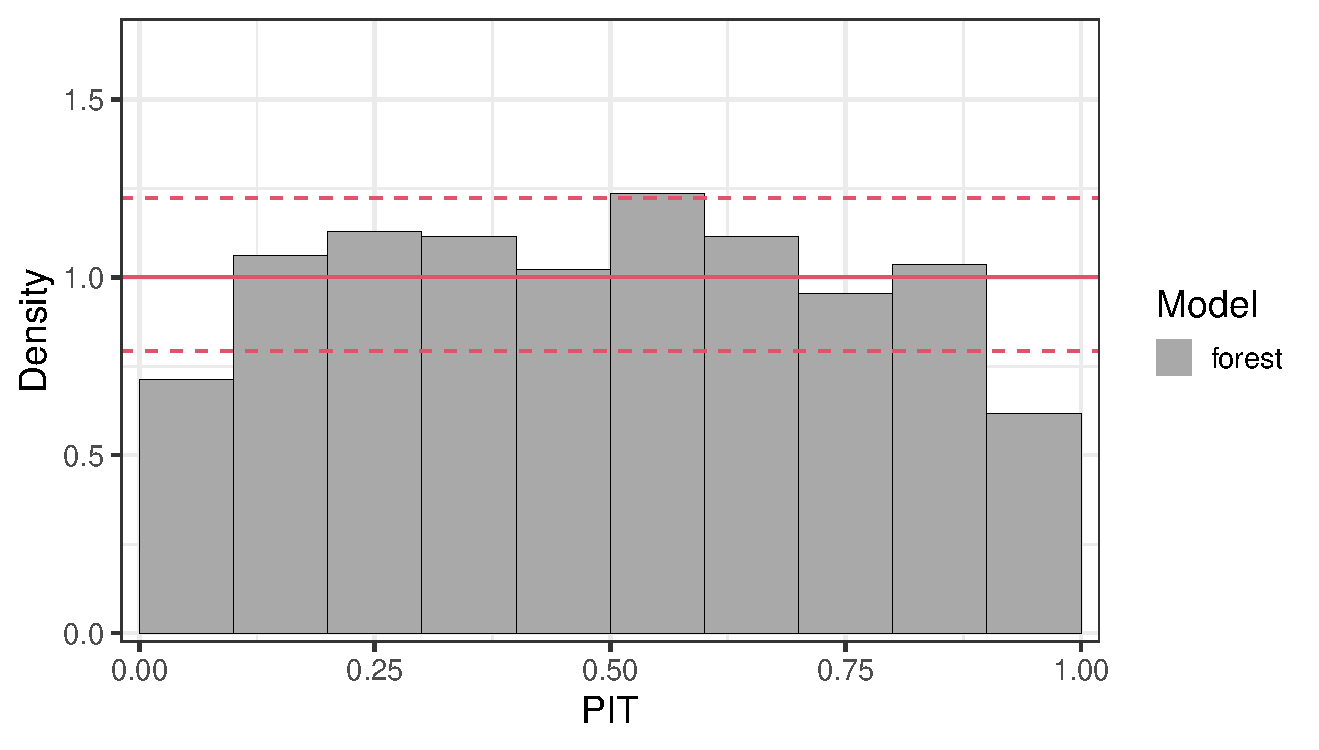
\includegraphics{slides-rain_topmodels_lm_pithist1_hist}
\end{center}

\end{frame}


%% SLIDE
\begin{frame}[fragile]
\addtocounter{framenumber}{-1}
\frametitle{Graphical assessment}

\vspace{-0.75em}

\textbf{Model comparison: PIT histogram}

\vspace{0.5em}

\begin{Schunk}
\begin{Sinput}
R> pithist(forest, plot = FALSE) |>
+    autoplot(legend = TRUE, style = "lines")
\end{Sinput}
\end{Schunk}

\begin{center}
\setkeys{Gin}{width=0.65\textwidth}
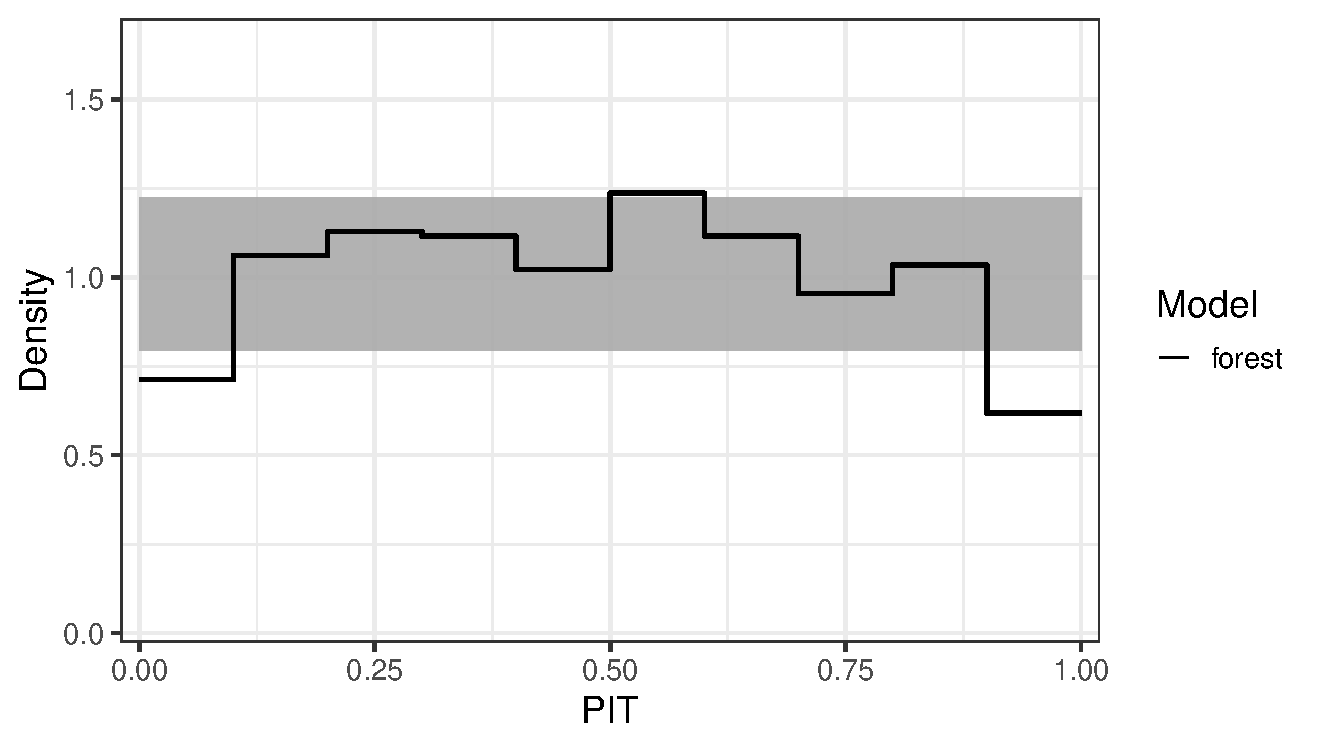
\includegraphics{slides-rain_topmodels_lm_pithist1_lines}
\end{center}

\end{frame}


%% SLIDE
\begin{frame}[fragile]
\addtocounter{framenumber}{-1}
\frametitle{Graphical assessment}

\vspace{-0.75em}

\textbf{Model comparison: PIT histogram}

\vspace{0.5em}

\begin{Schunk}
\begin{Sinput}
R> c(pithist(forest, plot = FALSE), pithist(linear, plot = FALSE)) |>
+    autoplot(legend = TRUE, style = "lines", single_graph = TRUE, col = 1:2)
\end{Sinput}
\end{Schunk}

\begin{center}
\setkeys{Gin}{width=0.65\textwidth}
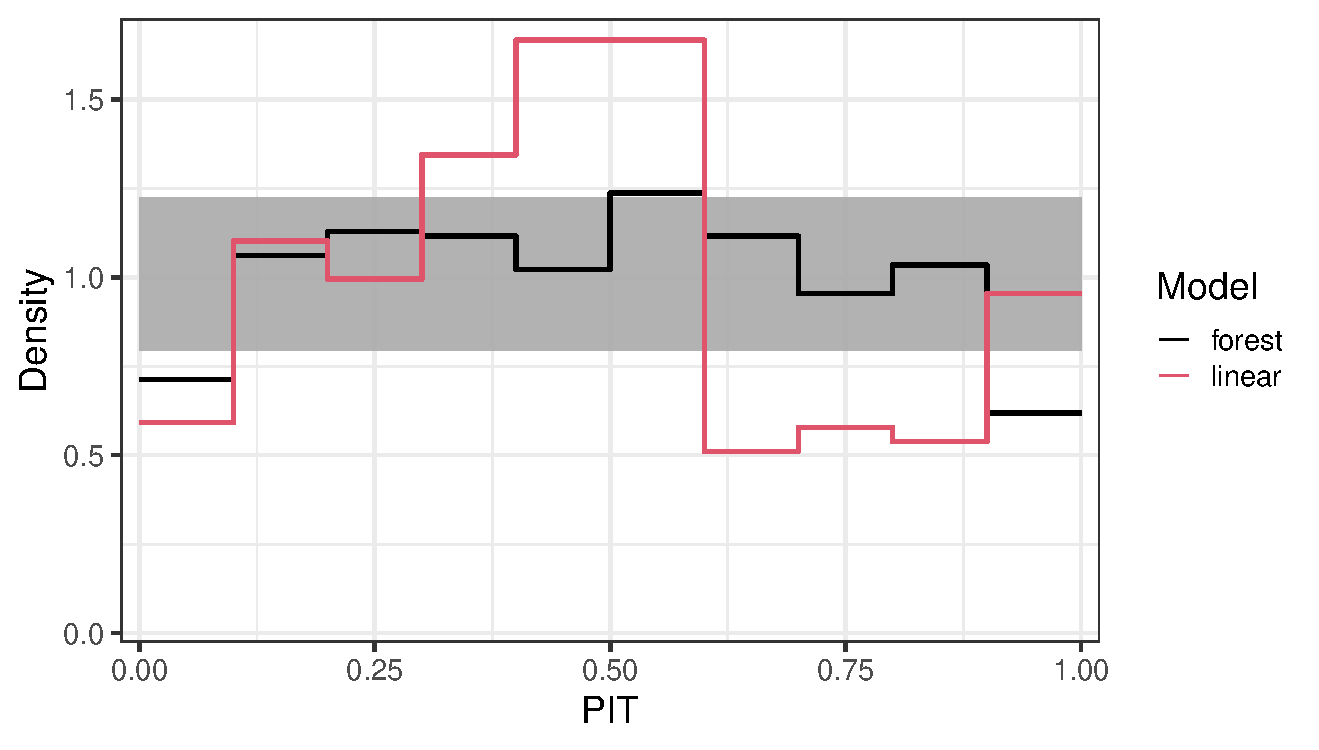
\includegraphics{slides-rain_topmodels_lm_pithist2}
\end{center}

\end{frame}


%% SLIDE
\begin{frame}[fragile]
\frametitle{Graphical assessment}

\vspace{-0.75em}

\textbf{Model comparison: Q-Q residuals plot}

\vspace{0.5em}

\begin{Schunk}
\begin{Sinput}
R> qqrplot(forest, plot = FALSE) |>
+    autoplot(legend = TRUE)
\end{Sinput}
\end{Schunk}

\begin{center}
\setkeys{Gin}{width=0.65\textwidth}
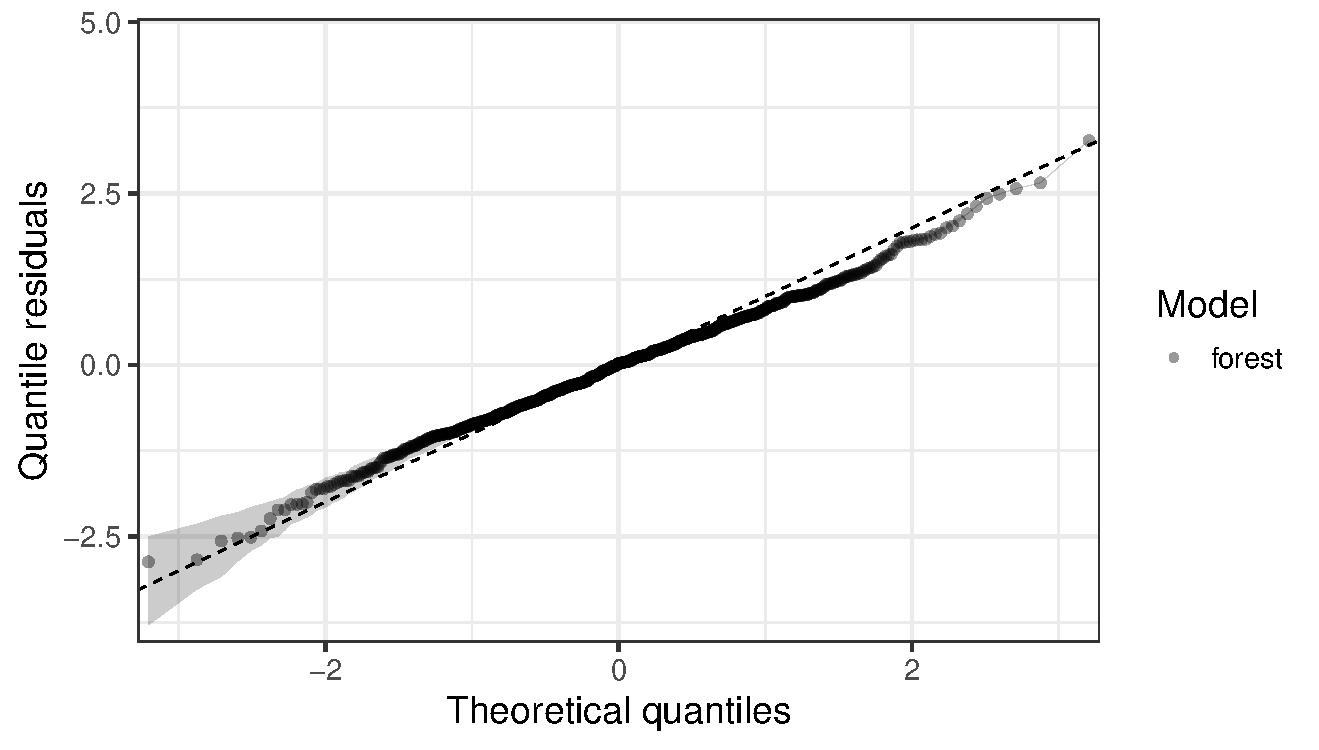
\includegraphics{slides-rain_topmodels_lm_qqrplot1}
\end{center}

\end{frame}


%% SLIDE
\begin{frame}[fragile]
\addtocounter{framenumber}{-1}
\frametitle{Graphical assessment}

\vspace{-0.75em}

\textbf{Model comparison: Q-Q residuals plot}

\vspace{0.5em}

\begin{Schunk}
\begin{Sinput}
R> c(qqrplot(forest, plot = FALSE), qqrplot(linear, plot = FALSE)) |>
+    autoplot(legend = TRUE, single_graph = TRUE, col = 1:2)
\end{Sinput}
\end{Schunk}

\begin{center}
\setkeys{Gin}{width=0.65\textwidth}
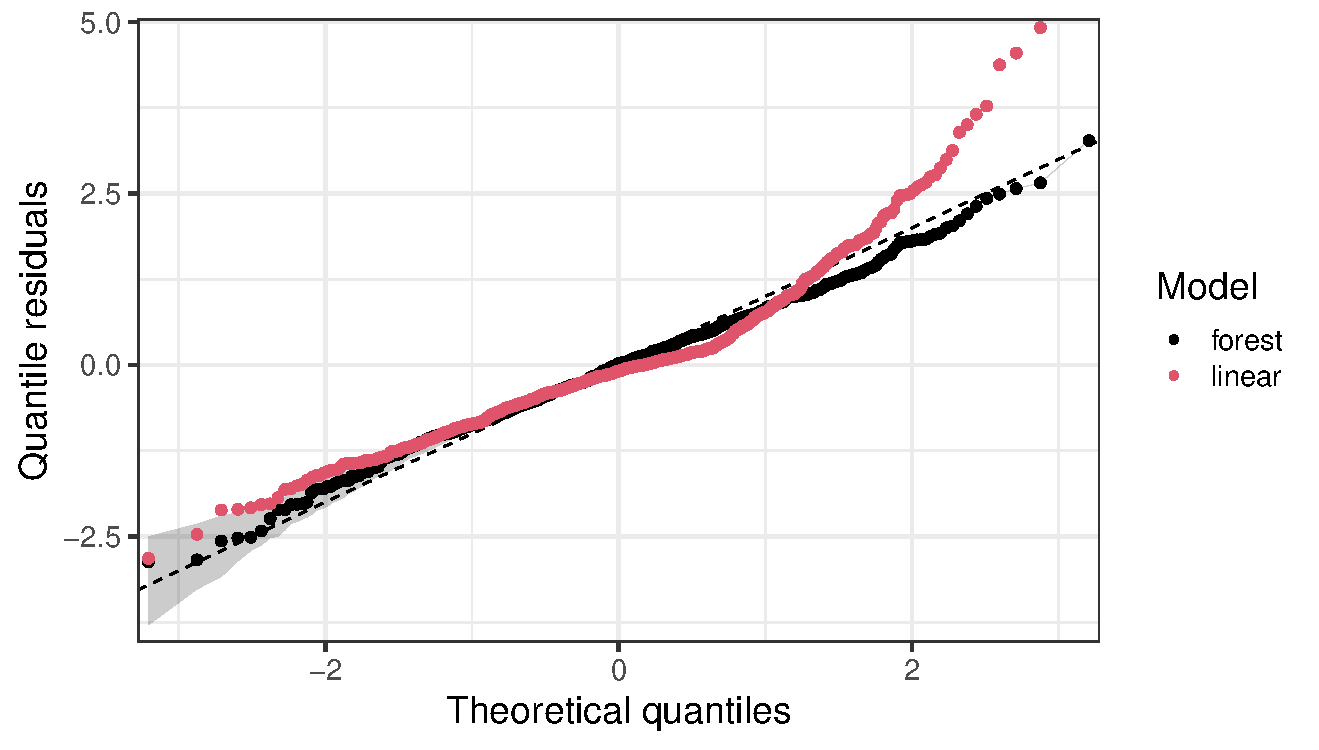
\includegraphics{slides-rain_topmodels_lm_qqrplot2}
\end{center}

\end{frame}

 
% %% SLIDE
% \begin{frame}[fragile]
% \frametitle{Graphical assessment}
% 
% \vspace{-0.75em}
% 
% \textbf{Model comparison: Reliability diagram}
% 
% \vspace{0.5em}
% 
% <<echo=TRUE,eval=FALSE>>=
% reliagram(forest, thresholds = 0.1, plot = FALSE) |>
%   autoplot(legend = TRUE, add_hist = FALSE, add_info = FALSE)
% @
% 
% \begin{center}
% \setkeys{Gin}{width=0.65\textwidth}
% <<rain_topmodels_lm_reliagram1, fig=TRUE, echo=FALSE, height=5., width=8.8>>=
% autoplot(c(forest = rel1_df1), legend = TRUE, add_hist = FALSE, add_info = FALSE)
% @
% \end{center}
% 
% \end{frame}
% 
% 
% %% SLIDE
% \begin{frame}[fragile]
% \addtocounter{framenumber}{-1}
% \frametitle{Graphical assessment}
% 
% \vspace{-0.75em}
% 
% \textbf{Model comparison: Reliability diagram}
% 
% \vspace{0.5em}
% 
% <<echo=TRUE,eval=FALSE>>=
% c(reliagram(forest, thr = 0.1, plot = F), reliagram(linear, thr = 0.1, plot = F)) |>
%   autoplot(legend = TRUE, single_graph = TRUE, col = 1:2, confint = 1:2)
% @
% 
% \begin{center}
% \setkeys{Gin}{width=0.65\textwidth}
% <<rain_topmodels_lm_reliagram2, fig=TRUE, echo=FALSE, height=5., width=8.8>>=
% autoplot(c(forest = rel1_df1, linear = rel1_lm1),
%           single_graph = TRUE, legend = TRUE, col = 1:2, confint = c(1:2))
% @
% \end{center}
% 
% \end{frame}
 

%-------------------------------------------------------------------
\subsection{Software}
%-------------------------------------------------------------------

%% SLIDE
\begin{frame}
\frametitle{Software}
\vspace{-0.75em}
\textbf{disttree:} available on R-Forge at\\

\medskip

\small{\url{https://R-Forge.R-project.org/projects/partykit/pkg/disttree/}}

\bigskip
\medskip

\textbf{Concept:} Fusion of tree-based models with distributional modeling.

\bigskip
\medskip

\textbf{Main functions:}

\medskip

\begin{tabular}{ll}
\code{distfit}    & Distributional fits (ML, \code{gamlss.family}/custom \code{list}).\\
& No covariates. \\
\code{disttree}   & Distributional trees (\code{ctree}/\code{mob} + \code{distfit}).\\
& Covariates as partitioning variables. \\
\code{distforest} & Distributional forests (ensemble of \code{disttree}s).\\
& Covariates as partitioning variables.
\end{tabular}

\end{frame}


%% SLIDE
\begin{frame}
\frametitle{Software}
\vspace{-0.75em}
\textbf{topmodels}: available on R-Forge at\\

\medskip

\small{\url{https://topmodels.R-Forge.R-project.org/}}\\ 

\bigskip
\medskip

\textbf{Concept:} Unifying toolbox for probabilistic forecasts and graphical model assessment.

\bigskip
\medskip

\textbf{Main functions:}

\medskip

\begin{tabular}{ll}
\code{procast}    & Probabilistic forecasts (\code{(g)lm}, \code{crch}, \code{disttree}, more to come).\\
& Computation of probabilities, densities, scores, and Hessians. \\
\code{rootogram}, \code{pithist}, \dots  & Plotting rootograms, PIT histograms, \dots \\
% \code{reliagram}, \code{qqrplot}, \dots   & reliability diagrams, (randomized) Q-Q plots, \dots.\\
\code{plot, autoplot}   & Generic \code{plot}, \code{autoplot} function.%\\
% \code{c}   & Generic \code{concatenate} function to plot combined objects.
\end{tabular}

\bigskip
\medskip

\end{frame}

%-------------------------------------------------------------------
\subsection{References}
%-------------------------------------------------------------------

%% SLIDE
\begin{frame}
\frametitle{References}

\footnotesize

Schlosser L, Hothorn T, Stauffer R, Zeileis A (2019).
\dquote{Distributional Regression Forests for Probabilistic Precipitation Forecasting in Complex Terrain.}
\emph{The Annals of Applied Statistics}, \textbf{13}(3), 1564--1589.
\doi{10.1214/19-AOAS1247}

\medskip

Lang MN, Zeileis A \emph{et al.} (2021).
\dquote{topmodels: Infrastructure for Inference and Forecasting in Probabilistic Models.}
\emph{R package version 0.1-0}.
\url{https://topmodels.R-Forge.R-project.org/}

\medskip

Hothorn T, Zeileis A (2015).
 \dquote{{partykit}: A Modular Toolkit for Recursive Partytioning in \textsf{R}.}
 \emph{Journal of Machine Learning Research},
 \textbf{16}, 3905--3909.
 \url{http://www.jmlr.org/papers/v16/hothorn15a}

% \bigskip
% \bigskip
% 
% Dunn PK, Smyth GK (1996).
% \dquote{Randomized Quantile Residuals.}
% \emph{Journal of Computational and Graphical Statistics}, \textbf{5}(3), 236--244.
% \doi{10.2307/1390802}
% 
% \medskip
% 
% Hothorn T, Hornik K, Zeileis A (2006).
%  \dquote{Unbiased Recursive Partitioning: A Conditional Inference Framework.}
%  \emph{Journal of Computational and Graphical Statistics},
%  \textbf{15}(3), 651--674.
%  \doi{10.1198/106186006X133933}
%  
% \medskip
% 
% Kleiber C, Zeileis A (2016).  
% \dQuote{Visualizing Count Data Regressions Using Rootograms.} 
% \emph{The American Statistician}, 
% \textbf{70}(3), 296--303.
% \doi{10.1080/00031305.2016.1173590}
% 
% \medskip
% Lang MN, Schlosser L, Hothorn T, Georg JM, Stauffer R, and Zeileis A (2020).
% \dquote{Circular Regression Trees and Forests with an Application to Probabilistic Wind Direction Forecasting.}
% \emph{Journal of the Royal Statistical Society C}, \textbf{69}(5), 1357--1374.
%  \doi{10.1111/rssc.12437}
%  
% \medskip
% 
% Zeileis A, Hothorn T, Hornik K (2008).
%  \dquote{Model-Based Recursive Partitioning.}
%   \emph{Journal of Computational and Graphical Statistics},
%   \textbf{17}(2), 492--514.
%   \doi{10.1198/106186008X319331}

\end{frame}


%% SLIDE
%%%
\title[]{\large{\color{uibkgraym}\url{https://topmodels.R-Forge.R-project.org/}}}
\author[]{\footnotesize \faEnvelope\,\,\href{mailto:moritz.lang@uibk.ac.at}{moritz.lang@uibk.ac.at} \hspace{1em} \faTwitter\,\href{https://twitter.com/MoritzNLang}{MoritzNLang}}
\URL{}

\section{Thank you}


% %-------------------------------------------------------------------
% \subsection{Appendix}
% %-------------------------------------------------------------------
% \backupbegin
% 
% %% SLIDE
% \begin{frame}
% ~~~
% \end{frame}
% 
% 
% %% SLIDE
% \begin{frame}
% \frametitle{Adaptive local likelihood estimation}
% \vspace{-0.75em}
% 
% \textbf{Parameter estimator} for \only<1-3>{\textbf{a global}}\only<4->{\textbf{an adaptive local}}\\ model with learning data \only<1>{$\{y_i\}_{i=1,\ldots,n}$}\only<2->{$\{(y_i,\mathbf{x}_i)\}_{i=1,\ldots,n}$} :
% 
% \[
% \hat{\theta}\visible<2->{(\mathbf{x})} =  \argmax_{\theta \in \Theta} \sum_{i=1}^n \visible<2->{w_i(\mathbf{x}) \cdot} \ell(\theta; y_i)
% \]
% 
% \medskip
% 
% \visible<3->{
% \textbf{Weights:}
% \begin{eqnarray*}
% w^{\text{base}}_i(\mathbf{x})   & = & 1 \\[0.2cm]
% \visible<4->{
% w^{\text{tree}}_i(\mathbf{x})   & = & \sum_{b=1}^B I((\mathbf{x}_i \in \mathcal{B}_b) \land (\mathbf{x} \in \mathcal{B}_b)) \\[0.1cm]
% \visible<5->{
% w^{\text{forest}}_i(\mathbf{x}) & = & \frac{1}{T} \sum_{t=1}^T \sum_{b=1}^{B^t} \frac{I((\mathbf{x}_i \in \mathcal{B}^t_b) \land (\mathbf{x} \in \mathcal{B}^t_b))}{|\mathcal{B}^t_b|}
% \end{eqnarray*}
% }}}
% \end{frame}
% 
% %% SLIDE
% \begin{frame}[fragile]
% \frametitle{Application}
% \vspace{-0.75em}
% 
% \textbf{One station:}
% \begin{itemize}
% \item Learn forest model on data from 24 years.
% \item Evaluate on 4 years.
% \item 10 times 7-fold cross validation.
% \end{itemize}
% 
% \bigskip
% 
% \textbf{Benchmark:} Against other heteroscedastic censored Gaussian models.
% \begin{itemize}
% \item \emph{Ensemble MOS:} Linear predictors using only total precipitation.
% \item \emph{Prespecified GAMLSS:} Variable selection based on expert knowledge.
% \item \emph{Boosted GAMLSS:} Automatic variable selection.
% \end{itemize}
% 
% \bigskip
% 
% \textbf{Evaluation:} Continuous ranked probability skill score.
% \end{frame}
% 
% 
% %% R CHUNK FOR NEXT SLIDE
% <<echo=FALSE, results=hide>>=
% #### cross validation rain
% if(file.exists("Data/crps_cross.rda")){
%   load("Data/crps_cross.rda")
% } else {
%   
%   nrep_cross <- 10
%   seed <- 7
%   
%   res_cross <- mclapply(1:nrep_cross,
%                         function(i){
%                           
%                           set.seed(seed*i)
%                           
%                           # randomly split data in 7 parts each including 4 years
%                           years <- 1985:2012
%                           testyears <- list()
%                           for(j in 1:7){
%                             testyears[[j]] <- sample(years, 4, replace = FALSE)
%                             years <- years[!(years %in% testyears[[j]])]
%                           }
%                           
%                           #crps <- matrix(nrow = 7, ncol = 7)
%                           reslist <- list()
%                           for(k in 1:7){
%                             test <- testyears[[k]]
%                             train <- c(1985:2012)[!c(1985:2012) %in% test]
%                             
%                             res <- evalmodels(station = "Axams",
%                                               train = train,
%                                               test = test,
%                                               gamboost_cvr = TRUE)
%                             
%                             #crps[k,] <- res$crps
%                             reslist[[k]] <- res
%                           }
%                           
%                           #colnames(crps) <- names(res$crps)
%                           return(reslist)
%                         },
%                         mc.cores = detectCores() - 1
%   )
%   
%   # extract CRPS
%   crps_cross <- matrix(nrow = nrep_cross, ncol = 7)
%   # loop over all repetitions
%   for(i in 1:length(res_cross)){
%     #loop over all 7 folds (for 7 methods)
%     crps_cross_int <- matrix(nrow = length(res_cross[[1]]), ncol = 7)
%     for(j in 1:length(res_cross[[1]])){
%       crps_cross_int[j,] <- res_cross[[i]][[j]]$crps
%     }
%     crps_cross[i,] <- colMeans(crps_cross_int, na.rm = TRUE)
%   }
%   colnames(crps_cross) <- names(res_cross[[1]][[1]]$crps) 
%   
%   save(crps_cross, file = "Data/crps_cross.rda")
% }
% @
% 
% %% SLIDE
% \begin{frame}[fragile]
% \frametitle{Application}
% \begin{center}
% \vspace*{-0.6cm}
% \setkeys{Gin}{width=0.7\textwidth}
% <<rain_cross_axams_crps_skills_score_with_title, fig=TRUE, echo=FALSE, height=5.6, width=6.8>>=
% #par(mar = c(2.5,2,1,2))
% boxplot(1 - crps_cross[,c(2,3,4)] / crps_cross[,6], ylim = c(-0.005, 0.065),
%         names = c("Distributional forest", "Prespecified GAMLSS", "Boosted GAMLSS"),
%         main = "Cross validation (with reference model EMOS)",
%         cex.main=1.4,
%         cex.lab=1.2,
%         ylab = "CRPS skill score", col = "lightgray") 
% abline(h = 0, col = pal["EMOS"], lwd = 2)
% @
% \end{center}
% \end{frame}
% 
% %% SLIDE
% \begin{frame}[fragile]
% \frametitle{Application}
% \vspace{-0.75em}
% \textbf{For all 95 stations:}
% 
% \begin{itemize}
% \item Learn forest model on data from 24 years (1985--2008).
% \item Evaluate on 4 years (2009--2012).
% \item Benchmark against other heteroscedastic censored Gaussian models.
% \end{itemize}
% 
% \end{frame}
% 
% 
% %% R CHUNK FOR NEXT SLIDE
% <<echo = FALSE>>=
% #### prediction over all stations 24 - 4
% if(file.exists("Data/crps_24to4_all.rda")){
%   load("Data/crps_24to4_all.rda")
% } else {
%   
%   data("StationsTyrol")
%   stations <- StationsTyrol$name
%   test <- 2009:2012
%   train <- 1985:2008
%   
%   
%   res_24to4_all <- mclapply(1:length(stations),
%                             function(i){
%                               
%                               set.seed(7)
%                               
%                               res <- evalmodels(station = stations[i],
%                                                 train = train,
%                                                 test = test,
%                                                 gamboost_cvr = TRUE)
%                               
%                               return(res)
%                             },
%                             mc.cores = detectCores() - 1
%   )
%   
%   # extract crps
%   crps_24to4_all <- matrix(nrow = length(stations), ncol = 7)
%   # loop over all stations
%   for(i in 1:length(stations)){
%     crps_24to4_all[i,] <- res_24to4_all[[i]]$crps
%   }
%   
%   colnames(crps_24to4_all) <- names(res_24to4_all[[1]]$crps)
%   rownames(crps_24to4_all) <- stations
%   
%   save(crps_24to4_all, file = "Data/crps_24to4_all.rda")
% }
% 
% 
% # skill score
% s <- 1 - crps_24to4_all[, 2:4]/crps_24to4_all[,6] 
% colnames(s) <- c("Distributional forest", "Prespecified GAMLSS", "Boosted GAMLSS")
% 
% 
% ## prepare data for map which shows where distforest performed better than gamlss or gamboostLSS based on the crps
% 
% crps_map <- crps_24to4_all[,c("distforest", "gamlss", "gamboostLSS", "emos_log")]  
% 
% # best method
% bst <- apply(crps_map, 1, which.min)
% 
% # distance of forest to best other method
% dst <- crps_map[,1] - crps_map[cbind(1:nrow(crps_map), apply(crps_map[, -1], 1, which.min) + 1)]
% 
% # breaks/groups
% brk <- c(-0.1, -0.05, -0.005, 0.005, 0.05, 0.1)
% #brk <- c(-0.1, -0.05, -0.01, 0.01, 0.05, 0.1)
% grp <- cut(dst, breaks = brk)
% 
% # HCL colors (relatively flashy, essentially CARTO Tropic)
% clr <- colorspace::diverging_hcl(5, h = c(130, 320), c = 70, l = c(50, 90), power = 1.3)
% 
% 
% library("raster") # dem (digital elevation model)
% library("sp")     # gadm www.gadm.org/country
% 
% data("StationsTyrol", package = "RainTyrol")
% data("MapTyrol", package = "RainTyrol")
% # data(MapTyrol_border, package = "RainTyrol")
% # Create SpatialPointsDataFrame from station list
% sp <- SpatialPointsDataFrame(subset(StationsTyrol,
%                                     select=c(lon,lat)),
%                              data = subset(StationsTyrol,
%                                            select = -c(lon,lat)),
%                              proj4string = crs(MapTyrol$RasterLayer))
% @
% 
% 
% %% SLIDE
% \begin{frame}[fragile]
% \frametitle{Precipitation forecasting}
% \begin{center}
% \vspace*{-0.5cm}
% 
% \setkeys{Gin}{width=0.8\textwidth}
% <<map, fig=TRUE, echo=FALSE, width=10, height=6.5>>=
% 
%   ## plot map of Tyrol with all 95 observations
%   layout(cbind(1, 2), width = c(9, 1))
%   par(mar = c(5,4,4,0.1))
%   raster::image(MapTyrol$RasterLayer, col = rev(gray.colors(100)),
%                 main="Stations in Tyrol", ylab = "Latitude", xlab = "Longitude", 
%                 xlim = c(9.8,13.2), 
%                 ylim = c(46.6, 47.87))
%   plot(MapTyrol$SpatialPolygons, add = TRUE)
%   points(sp[70,], pch = 19, col = "black", cex = 1.85)
%   points(sp, pch = c(21, 24, 25, 22)[bst], bg = clr[grp], col = "black", las = 1, cex = 1.5)
%   legend(x = 9.8, y = 47.815, pch = c(21, 24, 25, 22), legend = c("Distributional forest", "Prespecified GAMLSS", "Boosted GAMLSS", "EMOS"), cex = 1, bty = "n")
%   text(x = 10.3, y = 47.82, labels = "Models with lowest CRPS")
%   mtext("CRPS\ndifference", side=4, las = TRUE, at = c(x = 13.5, y = 47.76), line = 0.3)
%   par(mar = c(0.5,0.2,0.5,2.3))
%   ## legend
%   plot(0, 0, type = "n", axes = FALSE, xlab = "", ylab = "",
%        xlim = c(0, 1), ylim = c(-0.2, 0.2), xaxs = "i", yaxs = "i")
%   rect(0, brk[-6], 0.5, brk[-1], col = rev(clr))
%   axis(4, at = brk, las = 1, mgp=c(0,-0.5,-1))
% 
% 
% @
% \end{center}
% \end{frame}
% 
% \backupend

\end{document}
